\documentclass{ltxdoc}

\EnableCrossrefs
\CodelineIndex
\RecordChanges

\usepackage{mdframed}
\usepackage{minted}
\usepackage{luakeys}
\usepackage{luakeys-debug}
\usepackage{multicol}
\usepackage{luacode}
\usepackage{syntax}
\usepackage{graphicx}

\usemintedstyle{friendly}
\BeforeBeginEnvironment{minted}{\begin{mdframed}}
\AfterEndEnvironment{minted}{\end{mdframed}}
\setminted{
  breaklines=true,
  fontsize=\footnotesize,
  style=manni,
}
\def\lua#1{\mintinline{lua}|#1|}
\def\latex#1{\mintinline{latex}|#1|}

\NewDocumentCommand { \InputLatex } { O{} m } {
  \begin{mdframed}
  \inputminted[linenos=false,#1]{latex}{examples/#2}
  \end{mdframed}
}

\NewDocumentCommand { \InputLua } { O{} m } {
  \begin{mdframed}
  \inputminted[linenos=false,#1]{lua}{examples/#2}
  \end{mdframed}
}

\catcode`_=12
\def\DefaultOpt#1{%
  \texttt{\directlua{
    tex.print(luakeys.print_default('opts', '#1'))
  }}%
}

\def\DefaultOptDescription#1{
\noindent
The default value of the option “\texttt{#1}” is:
\DefaultOpt{#1}.
}

\begin{document}

\providecommand*{\url}{\texttt}

\title{The \textsf{luakeys} package}
\author{%
  Josef Friedrich\\%
  \url{josef@friedrich.rocks}\\%
  \href{https://github.com/Josef-Friedrich/luakeys}
       {github.com/Josef-Friedrich/luakeys}%
}
\date{0.10.0 from 2022/12/16}

\maketitle

\vfill

\InputLua[firstline=4,lastline=7]{first-page.lua}

\noindent
Result:

\begin{center}
\begin{minted}{lua}
{
  ['level1'] = {
    ['level2'] = {
      ['naked'] = true,
      ['dim'] = 1864679,
      ['bool'] = false,
      ['num'] = -0.001,
      ['str'] = 'lua,{}',
    }
  }
}
\end{minted}
\end{center}

\vfill

\strut

\newpage

\tableofcontents

\newpage

% \section{Einführung}
\section{Introduction}

\noindent
% |luakeys| ist ein Lua-Modul / Lua\TeX package, das wie die Pakete ...
% Schlüssel-Wert-Optionen analysieren kann.
|luakeys| is a Lua module / Lua\TeX package that can parse key-value
options like the \TeX{} packages
\href{https://www.ctan.org/pkg/keyval}{keyval},
\href{https://www.ctan.org/pkg/kvsetkeys}{kvsetkeys},
\href{https://www.ctan.org/pkg/kvoptions}{kvoptions},
\href{https://www.ctan.org/pkg/xkeyval}{xkeyval},
\href{https://www.ctan.org/pkg/pgfkeys}{pgfkeys} etc.
%
% |luakeys|, erfüllt diese Aufgabe jedoch, indem es die Sprache Lua
% verwendet und nicht auf \TeX{} angewiesen ist.
|luakeys|, however, accomplishes this task by using the Lua language and
doesn’t rely on \TeX{}.
%
% Deshalb kann dieses Paket nur mit der \TeX{}-Engine Lua\TeX{}
% verwendet werden.
Therefore this package can only be used with the
\TeX{} engine Lua\TeX{}.
%
% Da |luakeys| \href{http://www.inf.puc-rio.br/~roberto/lpeg/}{LPeg}
% verwendet, sollte der Parsing-Mechanismus ziemlich robust sein.
Since |luakeys| uses
\href{http://www.inf.puc-rio.br/~roberto/lpeg/}{LPeg}, the parsing
mechanism should be pretty robust.

% Der Artikel TUGboat
% \href{http://www.tug.org/tugboat/tb30-1/tb94wright-keyval.pdf}
% {“Implementing key–value input: An introduction” (Volume 30 (2009), No.
% 1)} von \emph{Joseph Wright} und \emph{Christian Feuersänger} gibt einen
% einen guten Überblick über die verfügbaren Key-Value-Pakete.
The TUGboat article
\href{http://www.tug.org/tugboat/tb30-1/tb94wright-keyval.pdf}
{“Implementing key–value input: An introduction” (Volume 30 (2009), No.
1)} by \emph{Joseph Wright} and \emph{Christian Feuersänger} gives a
good overview of the available key-value packages.

% Dieses Paket wäre ohne den Artikel
% \href{https://tug.org/TUGboat/tb40-2/tb125menke-lpeg.pdf}
% {"Parsing complex data formats in LuaTEX with LPEG" (Volume 40 (2019),
% No. 2)} nicht möglich gewesen.
This package would not be possible without the article
\href{https://tug.org/TUGboat/tb40-2/tb125menke-lpeg.pdf}
{“Parsing complex data formats in LuaTEX with LPEG” (Volume 40 (2019),
No. 2)}.

\subsection{Pros of \texttt{luakeys}}

\begin{itemize}
% \item Schlüssel-Wert-Paare können unabhängig vom Makro-Paket (latex or
% context) analysiert werden.
\item Key-value pairs can be parsed independently of the macro
collection (\LaTeX{} or Con\TeX{}t).

% \item Sogar in Plain LuaTex können Schlüssel analysiert werden
\item Even in plain Lua\TeX{} keys can be parsed.

% \item |luakeys| kann mit ineinander verschachtelten listen an
% Schlüssel-Wert-Paaren umgehen, d. h. es kann mit einer rekursiven
% Datenstruktur an Schlüssel umgehen.
\item |luakeys| can handle nested lists of key-value pairs, i.e. it can
handle a recursive data structure of keys.

% \item Schlüssel müssen nicht, aber können definiert werden.
\item Keys do not have to be defined, but can they can be defined.
\end{itemize}

\subsection{Cons of \texttt{luakeys}}

\begin{itemize}
% \item Das Packet funktioniert nur in der Verbindung mit Lua\TeX.
\item The package works only in combination with Lua\TeX.

% \item Du musst zwei Sprachen beherrschen: \TeX{} und Lua.
\item You need to know two languages: \TeX{} and Lua.
\end{itemize}

%-----------------------------------------------------------------------
%
%-----------------------------------------------------------------------

% \section{Wie das Paket geladen wird}
\section{How the package is loaded}

%%
%
%%

\subsection{Using the Lua module \texttt{luakeys.lua}}

% Die Kernfunktionalität dieses Pakets ist in Lua realisiert.
The core functionality of this package is realized in Lua.
%
% Sie können also |luakeys| auch ohne die Wrapper-Dateien
% \texttt{luakeys.sty} und \texttt{luakeys.tex} verwenden.
So you can use |luakeys| even without using the wrapper files
|luakeys.sty| and |luakeys.tex|.

\InputLatex{loading/lua.tex}

%%
%
%%

\subsection{Using the Lua\LaTeX{} wrapper \texttt{luakeys.sty}}

% Der Paketmanager MikTeX lädt beispielsweise Pakete erst bei Bedarf
% herunter.
For example, the MiK\TeX{} package manager downloads packages only when
needed.
%
% Es wurde berichtet, dass dieser automatische Download nur mit Hilfe
% der Hüll-Dateien funktioniert.
It has been reported that this automatic download only works with this
wrapper files.
%
% Wahrscheinlich hält MiK\TeX nach einem Auftreten des LaTeX macros
% “\latex{\usepackage{luakeys}} ”Ausschau.
Probably MiK\TeX{} is searching for an occurrence of the \LaTeX{} macro
“\latex{\usepackage{luakeys}}”.
%
% Die mitgelieferte Lua\LaTeX{}-Datei ist recht klein:
The supplied Lua\LaTeX{} file is quite small:

\begin{minted}{latex}
\NeedsTeXFormat{LaTeX2e}
\ProvidesPackage{luakeys}
\directlua{luakeys = require('luakeys')}
\end{minted}

\noindent
% Es lädt das Lua-Modul in die globale Variable \texttt{luakeys}.
It loads the Lua module into the global variable \texttt{luakeys}.

\InputLatex{loading/tex-latex.tex}

%%
%
%%

% \subsection{Verwendung des Plain-Lua\TeX{}-Hüllpakets
% \texttt{luakeys.tex}}
\subsection{Using the plain Lua\TeX{} wrapper \texttt{luakeys.tex}}

% Noch kleiner ist die Datei \texttt{luakeys.tex}.
Even smaller is the file \texttt{luakeys.tex}.
%
% Sie besteht aus nur einer Zeile:
It consists of only one line:

\begin{minted}{latex}
\directlua{luakeys = require('luakeys')}
\end{minted}

\noindent
% Es macht dasselbe wie das Lua\LaTeX{}-Hüllpacket und lädt das
% Lua-Modul \texttt{luakeys.lua} in die globale Variable
% \texttt{luakeys}.
It does the same as the Lua\LaTeX{} wrapper and loads the Lua module
\texttt{luakeys.lua} into the global variable \texttt{luakeys}.

\InputLatex{loading/tex-plain.tex}

%%%%%%%%%%%%%%%%%%%%%%%%%%%%%%%%%%%%%%%%%%%%%%%%%%%%%%%%%%%%%%%%%%%%%%%%
%
%%%%%%%%%%%%%%%%%%%%%%%%%%%%%%%%%%%%%%%%%%%%%%%%%%%%%%%%%%%%%%%%%%%%%%%%

\section{Lua interface / API}

% Das Lua-Modul exportiert diese Funktionen und Tabellen:
The Lua module exports this functions and tables:

\InputLua[firstline=3,lastline=15]{export.lua}

% Diese Dokumentation stellt nur die öffentlichen Funktionen und
% Tabellen vor.
This documentation presents only the public functions and tables.
%
% Um mehr über die privaten, nicht exportierten Funktionen zu erfahren,
% lesen Sie bitte die
% \href{https://josef-friedrich.github.io/luakeys/}{Quellcode
% Dokumentation}, die mit
% \href{http://stevedonovan.github.io/ldoc/}{LDoc} erstellt wurde.
To learn more about the private, not exported functions, please
read the \href{https://josef-friedrich.github.io/luakeys/}{source code
documentation}, which was created with
\href{http://stevedonovan.github.io/ldoc/}{LDoc}.

\subsection{Lua indentifier names}

% Das Projekt verwendet einige wenige Abkürzungen für Variablennamen,
% die hoffentlich für externe Leser eindeutig und bekannt sind.
The project uses a few abbreviations for variable names that are
hopefully unambiguous and familiar to external readers.

\begin{center}
\begin{tabular}{lll}
Abbreviation & spelled out & Example \\\hline
\lua{kv_string} & Key-value string & \lua{'key=value'} \\
\lua{opts} & Options (for the parse function) &
\lua{ { no_error = false } } \\
\lua{defs} & Definitions \\
\lua{def} & Definition \\
\lua{attr} & Attributes (of a definition) \\
\end{tabular}
\end{center}

\noindent
% Diese nicht abgekürzten Variablennamen werden häufig verwendet.
These unabbreviated variable names are commonly used.
\begin{center}
\begin{tabular}{ll}

\lua{result} &
% Das Endergebnis aller einzelnen Übersetzungs- und
% Normalisierungsschritte
The final result of all individual parsing and normalization steps. \\

\lua{unknown} &
% Ein Tabelle mit unbekannten, nicht definierten Schlüssel-Wert-Paaren
A table with unknown, undefinied key-value pairs. \\

\lua{raw} &
% Das unbearbeitete, rohe Ergebnis der LPeg-Syntaxanalyse.
The raw result of the Lpeg grammar parser. \\
\end{tabular}
\end{center}

%%
%
%%

\subsection{Function “\texttt{get_new_instance(): table}”}

% Über die Tabelle \lua{opts} können die  Standardoptionen global
% geändert werden.
The default options can be changed globally via the \lua{opts} table.
% Um zu verhindern, dass andere Module die Standardeinstellungen
% ändern, kann mit Hilfe der Funktion \lua{get_new_instance()} eine neue
% Instanz des Moduls \lua{luakeys} erzeugt werden.
To prevent another modules from changing the default settings, a new
instance of the  \lua{luakeys} module can be created using the
\lua{get_new_instance()} function.

\InputLua[firstline=3,lastline=4]{functions/get-new-instance.lua}

\noindent
% Die Funktion \lua{require()} gibt standardmäßig beim mehrmaligen
% Aufruf immer die gleiche Tabelle zurück.
The \lua{require()} function always returns the same table
when called multiple times.

\InputLua[firstline=14,lastline=17]{functions/get-new-instance.lua}

%%
%
%%

\subsection{Function “\texttt{parse(kv_string, opts): result, unknown,
raw}”}
\label{parse}

% Die Function parse ist die wichtigste Funktion des Pakets.
The function \lua{parse(kv_string, opts)} is the most important function
of the package.
%
%
% Sie konvertiert eine Schlüssel-Wert-Zeichenkette in eine Lua Tabelle.
It converts a key-value string into a Lua table.

\InputLatex{functions/parse/tex-latex.tex}

\noindent
In plain \TeX:

\InputLatex{functions/parse/tex-plain.tex}

\subsection{Options to configure the \texttt{parse} function}

\noindent
% Die Funktion \lua{parse} kann mit einer Optionstabelle aufgerufen
% werden.
The \lua{parse} function can be called with an options table.
% Diese Optionen werden unterstützt:
This options are supported: \catcode`_=12
\directlua{luakeys.print_names('opts')}

\InputLua[firstline=5,lastline=94]{opts/all-opts.lua}

\noindent
% Die Optionen können auch global über die exportierte Tabelle
% \lua{opts} gesetzt werden:
The options can also be set globally using the exported table
\lua{opts}:

\InputLua[firstline=4,lastline=4]{opts/exported-default-opts.lua}

\InputLua[firstline=10,lastline=11]{opts/exported-default-opts.lua}

%%
%
%%

\subsubsection{Option “\texttt{assignment_operator}”}
\label{option:assignment-operator}
\label{options-delimiter}

The option \lua{assignment_operator} configures the delimiter that
assigns a value to a key. The default value of this option is
\texttt{"="}.

The code example below demonstrates all six delimiter related options.

\InputLua[firstline=4,lastline=13]{opts/delimiters.lua}

\begin{tabular}{ll}
\textbf{Delimiter options} & \textbf{Section} \\
assignment_operator & \ref{option:assignment-operator}\\
group_begin & \ref{option:group-begin}\\
group_end & \ref{option:group-end}\\
list_separator & \ref{option:list-separator}\\
quotation_begin & \ref{option:quotation-begin}\\
quotation_end & \ref{option:quotation-end}\\
\end{tabular}

%%
%
%%

\subsubsection{Option “\texttt{convert_dimensions}”}

% Wenn Sie die Option \lua{convert_dimensions} auf \lua{true} setzen,
% erkennt |luakeys| die \TeX{}-Dimensionen und konvertiert sie mit Hilfe
% der die Funktion \lua{tex.sp(dim)} in scaled points.
If you set the option \lua{convert_dimensions} to \lua{true}, |luakeys|
detects the \TeX{} dimensions and converts them into scaled points using
the function \lua{tex.sp(dim)}.

\InputLua[firstline=4,lastline=7]{opts/convert-dimensions/true.lua}

\noindent
% Standardmäßig werden die Dimensionen nicht in skalierte Punkte
% umgewandelt.
By default the dimensions are not converted into scaled points.

\InputLua[firstline=4,lastline=9]{opts/convert-dimensions/false.lua}

\noindent
% Wenn Sie eine skalierte Punktzahl in einen Dimensionszeichenketten
% umwandeln möchten, können Sie das Modul
If you want to convert a scaled points number into a dimension string
you can use the module
\href{https://raw.githubusercontent.com/latex3/lualibs/master/lualibs-util-dim.lua}
{lualibs-util-dim.lua}.

\begin{minted}{lua}
require('lualibs')
tex.print(number.todimen(tex.sp('1cm'), 'cm', '%0.0F%s'))
\end{minted}

\DefaultOptDescription{convert_dimensions}

%%
%
%%

\subsubsection{Option “\texttt{debug}”}

% Wenn die Option \lua{debug} auf true gesetzt ist, wird die
% Ergebnistabelle in der Konsole ausgegeben.
If the option \lua{debug} is set to true, the result table is printed to
the console.

\InputLatex{opts/debug-latex.tex}

\begin{verbatim}
This is LuaHBTeX, Version 1.15.0 (TeX Live 2022)
...
(./debug.aux) (/usr/local/texlive/texmf-dist/tex/latex/base/ts1cmr.fd)
{
  ['three'] = true,
  ['two'] = true,
  ['one'] = true,
}
 [1{/usr/
local/texlive/2022/texmf-var/fonts/map/pdftex/updmap/pdftex.map}] (./debug.aux)
)
...
Transcript written on debug.log.
\end{verbatim}

\DefaultOptDescription{debug}

%%
%
%%

\subsubsection{Option “\texttt{default}”}
\label{option-default}

% Mit der Option \lua{default} kann angegeben werden, welchen Wert
% nackte Schlüssel (Schlüssel ohne Wert) erhalten. Diese Option hat
% keinen Einfluss auf Schlüssel mit Werten.
The option \lua{default} can be used to specify which value naked keys
(keys without a value) get. This option has no influence on keys with
values.

\InputLua[firstline=4,lastline=5]{opts/default.lua}

\noindent
% Standardmäßig erhalten nackte Schlüssel den Wert \lua{true}.
By default, naked keys get the value \lua{true}.

\InputLua[firstline=11,lastline=12]{opts/default.lua}

\DefaultOptDescription{default}

%%
%
%%

\subsubsection{Option “\texttt{defaults}”}
\label{options-defaults}

% Mit der Attribut „defaults“ kann nicht nur ein einiger Standardwert
% angegeben werden, sondern eine ganze Tabelle mit Standardwerten.
The option “defaults” can be used to specify not only one default value,
but a whole table of default values.
% Die Ergebnistabelle wird mit der Tabelle bestehend aus Standardwerten
% vereinigt.
The result table is merged into the defaults table.
% Werte aus der Tabelle mit Standardwerten werden von Werten der
% Ergebnistabelle überschrieben.
Values in the defaults table are
overwritten by values in the result table.

\InputLua[firstline=4,lastline=7]{opts/defaults.lua}

\DefaultOptDescription{defaults}

%%
%
%%

\subsubsection{Option “\texttt{defs}”}

% Für mehr Information wie Schlüssel definiert werden, lesen sie das
% kapitel 3.2
For more informations on how keys are defined, see section \ref{define}.
% Wenn sie die Option \lua{defs} verwenden, können sie auf den
% Aufruf der Funktion \lua{define} verzichten.
If you use the \lua{defs} option, you don't need to call the
\lua{define} function.
%
% Anstatt
Instead of ...

\InputLua[firstline=4,lastline=5]{opts/defs.lua}

\noindent
% können wir schreiben ..
we can write ...

\InputLua[firstline=11,lastline=13]{opts/defs.lua}

\DefaultOptDescription{defs}

%%
%
%%

\subsubsection{Option “\texttt{false_aliases}”}
\label{option:false-aliases}

% Mit den den Optionen \lua{true_aliases} and \lua{false_aliases} können
% die Zeichenketten festgelegt werden, die vom Parser als Wahrheitswerte
% erkannt werden.
The \lua{true_aliases} and \lua{false_aliases} options can be used to
specify the strings that will be recognized as boolean values by the
parser.
% Standardmäßig sind folgende Zeichenketten konfiguriert
The following strings are configured by default.

\InputLua[firstline=4,lastline=8]{opts/boolean-aliases.lua}

\InputLua[firstline=14,lastline=18]{opts/boolean-aliases.lua}

\InputLua[firstline=24,lastline=28]{opts/boolean-aliases.lua}

% Siehe Abschnitt \label{option:true-aliases} für die entsprechende
% Option.
See section \ref{option:true-aliases} for the corresponding option.

%%
%
%%

\subsubsection{Option “\texttt{format_keys}”}

% Mit Hilfe der Option \lua{format_keys} können die Schlüssel formatiert
% werden.
With the help of the option \lua{format_keys} the keys can be formatted.
% Die Werte dieser Option müssen in einer Tabelle angegeben werden.
The values of this option must be specified in a table.

\begin{description}
\item[lower]

% Um alle Schlüssel in \emph{Kleinbuchstaben} umzuwandeln, geben sie in
% der Optionentabelle \lua{lower} an.
To convert all keys to \emph{lowercase}, specify \lua{lower} in the
options table.

\InputLua[firstline=4,lastline=5]{opts/format-keys.lua}

\item[snake]

% Um alle Schlüssel in \emph{snake case} (Die Wörter sind durch
% Unterstriche getrennt) umzuwandeln, geben sie in der Optionentabelle
% \lua{snake} an.
To make all keys \emph{snake case} (The words are separated by
underscores), specify \lua{snake} in the options
table.

\InputLua[firstline=11,lastline=12]{opts/format-keys.lua}

\item[upper]

% Um alle Schlüssel in \emph{Grossbuchstaben} umzuwandeln, geben sie in
% der Optionentabelle \lua{upper} an.
To convert all keys to \emph{uppercase}, specify \lua{upper} in the
options table.

\InputLua[firstline=18,lastline=19]{opts/format-keys.lua}
\end{description}

% Sie können auch mehrere Formatierungsarten kombinieren.
You can also combine several types of formatting.

\InputLua[firstline=25,lastline=26]{opts/format-keys.lua}

\DefaultOptDescription{format_keys}

%%
%
%%

\subsubsection{Option “\texttt{group_begin}”}
\label{option:group-begin}

The option \lua{group_begin} configures the delimiter that marks the
beginning of a group. The default value of this option is \texttt{"\{"}.
A code example can be found in section \ref{options-delimiter}.

%%
%
%%

\subsubsection{Option “\texttt{group_end}”}
\label{option:group-end}

The option \lua{group_end} configures the delimiter that marks the end
of a group. The default value of this option is \texttt{"\}"}. A code
example can be found in section \ref{options-delimiter}.

%%
%
%%

\subsubsection{Option “\texttt{invert_flag}”}

% Wird ein nackter Schlüssel mit einem vorangestellten Ausrufezeichen versehen, so wird sein Standardwert invertiert.
If a naked key is prefixed with an exclamation mark, its default value
is inverted.
% Statt \lua{true} nimmt der Schlüssel jetzt den Wert \lua{falsch} an.
Instead of \lua{true} the key now takes the value \lua{false}.

\InputLua[firstline=4,lastline=5]{opts/invert-flat.lua}

\noindent
% Mit der Option \lua{invert_flag} kann dieses Invertierungszeichen
% geändert werden.
The \lua{invert_flag} option can be used to change this inversion
character.

\InputLua[firstline=11,lastline=12]{opts/invert-flat.lua}

\noindent
% Ist der Standardwert für nackte Schlüssel beispielweise auf \lua{false}
% gesetzt, so nehmen die mit dem Umkehrungszeichen versehenen nackten
% Schlüssel den Wert \lua{true} an.
For example, if the default value for naked keys is set to \lua{false},
the naked keys prefixed with the invert flat take the value \lua{true}.

\InputLua[firstline=18,lastline=19]{opts/invert-flat.lua}

\noindent
% Setzen sie die Option \lua{invert_flag} auf \lua{false}, um diese
% automatische Wertumkehrung zu deaktivieren.
Set the \lua{invert_flag} option to \lua{false} to disable this
automatic boolean value inversion.

\InputLua[firstline=25,lastline=26]{opts/invert-flat.lua}

%%
%
%%

\subsubsection{Option “\texttt{hooks}”}

% Die folgenden Hooks bzw. Callback-Funktionen ermöglichen es in den
% Verarbeitungsprozess der \lua{parse}-Function einzugreifen.
The following hooks or callback functions allow to intervene in the
processing of the \lua{parse} function.
%
% Die Funktionen sind in der Verarbeitungsreihenfolge aufgelistet.
The functions are listed in processing order.
%
% \lua{*_before_opts} bedeutet, dass die Hooks nach der LPeg
% Syntaxanalyse und vor dem Anwenden der Optionen ausgeführt
\lua{*_before_opts} means that the hooks are executed after the LPeg
syntax analysis and before the options are applied.
%
% Die Hooks \lua{*_before_defs} werden vor dem Anwenden der
% Schlüssel-Wert-Definitionen ausgeführt
The \lua{*_before_defs} hooks are executed before applying the key value
definitions.

\def\TmpSignature#1{
  {
    \scriptsize\texttt{ = #1}
  }
}

\def\TmpKeySignature{
  \TmpSignature{function(key, value, depth, current, result): key, value}
}
\def\TmpResultSignature{
  \TmpSignature{function(result): void}
}

\begin{enumerate}
\item \lua{kv_string} \TmpSignature{function(kv_string): kv_string}
\item \lua{keys_before_opts} \TmpKeySignature
\item \lua{result_before_opts} \TmpResultSignature
\item \lua{keys_before_def} \TmpKeySignature
\item \lua{result_before_def} \TmpResultSignature
\item (\lua{process}) (has to be definied using defs, see \ref{attr-process})
\item \lua{keys} \TmpKeySignature
\item \lua{result} \TmpResultSignature
\end{enumerate}

\paragraph{\texttt{kv_string}}

% Der Hook \lua{kv_string} wird als erste
% der Hook-Funktionen noch vor der LPeg-Syntax-Analyse aufgerufen.
The \lua{kv_string} hook is called as the first of the hook functions
before the LPeg syntax parser is executed.

\InputLua[firstline=4,lastline=11]{hooks/kv-string.lua}

\paragraph{\texttt{keys_*}}

% Die Hooks \lua{keys_*} werden rekursiv auf jeden Schlüssel in der
% aktuellen Ergebnistabelle aufgerufen.
The hooks \lua{keys_*} are called recursively on each key in the current
result table.
% Die Hook-Funktion muss zwei Werte zurückgeben: \lua{key, value}
The hook function must return two values: \lua{key, value}.
%
% Das folgende Beispiel gibt \lua{key} und \lua{value} unverändert
% zurück, sodass die Ergebnistabelle nicht verändert wird.
The following example returns \lua{key} and \lua{value} unchanged, so
the result table is not changed.

\InputLua[firstline=4,lastline=11]{hooks/keys-unchanged.lua}

\noindent
% Das nächste Beispiel demonstriert den dritten Parameter \lua{depth}
% der Hook-Funktion.
The next example demonstrates the third parameter \lua{depth} of the
hook function.

\InputLua[firstline=4,lastline=16]{hooks/keys-depth.lua}

\paragraph{\texttt{result_*}}

% Die Hooks \lua{result_*} werden einmal mit der aktuellen
% Ergebnistabelle als Parameter aufgerufen.
The hooks \lua{result_*} are called once with the current result table
as a parameter.

%%
%
%%

\subsubsection{Option “\texttt{list_separator}”}
\label{option:list-separator}

The option \lua{list_separator} configures the delimiter that separates
list items from each other. The default value of this option is
\texttt{","}. A code example can be found in section
\ref{options-delimiter}.

%%
%
%%

\subsubsection{Option “\texttt{naked_as_value}”}

% Mit Hilfe der Option \lua{naked_as_value} werden nackte Schlüssel
% nicht mit einem Standardwert versehen, sondern als Werte in die
% Lua-Tabelle abgelegt.
With the help of the option \lua{naked_as_value}, naked keys are not
given a default value, but are stored as values in a Lua table.

\InputLua[firstline=4,lastline=5]{opts/naked-as-value.lua}

\noindent
If we set the option \lua{naked_as_value} to \lua{true}:

\InputLua[firstline=11,lastline=14]{opts/naked-as-value.lua}

\DefaultOptDescription{naked_as_value}

%%
%
%%

\subsubsection{Option “\texttt{no_error}”}

% Standardmaßig wirft parse-Funktion einen Fehler, wenn es unbekannte
% Schlüssel gibt.
By default the parse function throws an error if there are unknown keys.
% Mit Hilfe der Option \lua{no_error} kann dies unterbunden werden.
This can be prevented with the help of the \lua{no_error} option.

\InputLua[firstline=5,lastline=6]{opts/no-error.lua}

\noindent
If we set the option \lua{no_error} to \lua{true}:

\InputLua[firstline=9,lastline=10]{opts/no-error.lua}

\DefaultOptDescription{no_error}

%%
%
%%

\subsubsection{Option “\texttt{quotation_begin}”}
\label{option:quotation-begin}

The option \lua{quotation_begin} configures the delimiter that marks the
beginning of a string. The default value of this option is
\texttt{'"'} (double quotes). A code example can be found in section
\ref{options-delimiter}.

%%
%
%%

\subsubsection{Option “\texttt{quotation_end}”}
\label{option:quotation-end}

The option \lua{quotation_end} configures the delimiter that marks the
end of a string. The default value of this option is \texttt{'"'}
(double quotes). A code example can be found in section
\ref{options-delimiter}.

%%
%
%%

\subsubsection{Option “\texttt{true_aliases}”}
\label{option:true-aliases}

See section \ref{option:false-aliases}.

%%
%
%%

\subsubsection{Option “\texttt{unpack}”}

% Mit Hilfe der Option \lua{unpack} werden alle Tabellen, die nur aus
% einem einzigen nackten Schlüssel bzw. einen einzigen alleinstehenden
% Wert bestehen, aufgelöst.
With the help of the option \lua{unpack}, all tables that consist of
only a single naked key or a single standalone value are unpacked.

\InputLua[firstline=4,lastline=5]{opts/unpack.lua}

\InputLua[firstline=11,lastline=12]{opts/unpack.lua}

\DefaultOptDescription{unpack}

%%
%
%%

\subsection{Function “\texttt{define(defs, opts): parse}”}
\label{define}

The \lua{define} function returns a \lua{parse} function (see
\ref{parse}).
The name of a key can be specified in three ways:

\begin{enumerate}
\item as a string.
\item as a key in a Lua table. The definition of the corresponding
key-value pair is then stored under this key.
\item by the “name” attribute.
\end{enumerate}

\InputLua[firstline=4,lastline=16]{functions/define.lua}

\noindent
% Bei verschachtelten Definitionen können nur die letzten beiden
% Möglichkeiten zur Angabe der Schlüsselnamen verwendet werden.
For nested definitions, only the last two ways of specifying the key
names can be used.

\InputLua[firstline=26,lastline=33]{functions/define.lua}

%-----------------------------------------------------------------------
%
%-----------------------------------------------------------------------

\subsection{Attributes to define a key-value pair}

% Die Definition eines Schlüssel-Wert-Paares kann mit Hilfe von
% verschiedenen Attributen vorgenommen werden.
The definition of a key-value pair can be made with the help of various
attributes.
%
% Der Name „Attribut“ für eine Option, einen Schlüssel, eine Eigenschaft
% (um nur einige Benennungsmöglichkeiten aufzuzählen) zur
% Schlüssel-Definition, wurde bewusst gewählt, um sie von den Optionen
% der Funktion \lua{parse} zu unterscheiden.
The name \emph{“attribute”} for an option, a key, a property ... (to
list just a few naming possibilities) to define keys, was deliberately
chosen to distinguish them from the options of the \lua{parse} function.
%
% Diese Attribute sind erlaubt.
These attributes are allowed:
\directlua{luakeys.print_names('attrs')}.
%
% Das folgende Codebeispiel listet alle Attribute auf, die verwendet
% werden können, um Schlüssel-Wert-Paare zu definieren.
The code example below lists all the attributes that can be used to
define key-value pairs.

\InputLua[firstline=5,lastline=46]{defs/all-attrs.lua}

%%
%
%%

\subsubsection{Attribute “\texttt{alias}”}

With the help of the \lua{alias} attribute, other key names can be used.
The value is always stored under the original key name. A single alias
name can be specified by a string ...

\InputLua[firstline=4,lastline=7]{defs/attrs/alias.lua}

\noindent
multiple aliases by a list of strings.

\InputLua[firstline=13,lastline=16]{defs/attrs/alias.lua}

%%
%
%%

\subsubsection{Attribute “\texttt{always_present}”}

% Die Option \lua{default} wird nur bei nackten Schlüsseln verwendet.
The \lua{default} attribute is used only for naked keys.

\InputLua[firstline=4,lastline=5]{defs/attrs/always-present.lua}

\noindent
% Wird die Option \lua{always_present} auf wahr gesetzt, wird der
% Schlüssel immer ins Ergebnis mit übernommen.
If the attribute \lua{always_present} is set to true, the key is always
included in the result. If no default value is definied, true is taken
as the value.

\InputLua[firstline=11,lastline=12]{defs/attrs/always-present.lua}

%%
%
%%

\subsubsection{Attribute “\texttt{choices}”}

% source: Python argparse documentation.
Some key values should be selected from a restricted set of choices.
These can be handled by passing an array table containing choices.

\InputLua[firstline=4,lastline=5]{defs/attrs/choices.lua}

\noindent
When the key-value pair is parsed, values will be checked, and an error
message will be displayed if the value was not one of the acceptable
choices:

\InputLua[firstline=13,lastline=15]{defs/attrs/choices.lua}

%%
%
%%

\subsubsection{Attribute “\texttt{data_type}”}

% source: Python argparse documentation.
The \lua{data_type} attribute allows type-checking and type conversions to
be performed.
%
% Folgende Datentypen werden unterstützt:
The following data types are supported:
\lua{'boolean'},
\lua{'dimension'},
\lua{'integer'},
\lua{'number'},
\lua{'string'}.
%
% Bei den drei Datentypen integer, number, dimension kann eine
% Typenumwandlung scheitern.
A type conversion can fail with the three data types
\lua{'dimension'},
\lua{'integer'},
\lua{'number'}.
%
% Dann wird eine Fehlermeldung ausgegeben.
Then an error message is displayed.

\InputLua[firstline=4,lastline=8]{defs/attrs/data-type.lua}
\InputLua[firstline=11,lastline=15]{defs/attrs/data-type.lua}

%%
%
%%

\subsubsection{Attribute “\texttt{default}”}

% Verwenden Sie das Attribut „\lua{default}“, um für jeden nackten Schlüssel
% einzeln einen Standardwert bereit zu stellen.
Use the \lua{default} attribute to provide a default value for each naked
key individually.
%
% Mit der globalen \lua{default} Option kann für alle nackten Schlüssel ein
% Standardwert vorgegeben werden.
With the global \lua{default} attribute (\ref{option-default}) a default
value can be specified for all naked keys.

\InputLua[firstline=4,lastline=9]{defs/attrs/default.lua}

%%
%
%%

\subsubsection{Attribute “\texttt{exclusive_group}”}

% Alle Schlüssel, die der gleichen ausschließenden Gruppe angehören,
% dürfen nicht gemeinsam angegeben werden.
All keys belonging to the same exclusive group must not be specified
together.
%
% Nur ein Schlüssel aus dieser Gruppe ist erlaubt.
Only one key from this group is allowed.
%
% Als Name für diese ausschließende Gruppe kann irgend ein beliebiger
% Wert verwendet werden.
Any value can be used as a name for this exclusive group.

\InputLua[firstline=4,lastline=9]{defs/attrs/exclusive-group.lua}

\noindent
% Werden mehrer Schlüssel der Gruppe angegeben, so wird eine
% Fehlermeldung geworfen.
If more than one key of the group is specified, an error message is
thrown.

\InputLua[firstline=21,lastline=23]{defs/attrs/exclusive-group.lua}

%%
%
%%

\subsubsection{Attribute “\texttt{opposite_keys}”}

% Die Option \lua{opposite_keys} ermöglicht es, gegensätzliche (nackte)
% Schlüssel in Wahrheitswerte umzuwandeln und diesen Wahrheitswert unter
% einem Zielschlüssel zu speichern.
The \lua{opposite_keys} attribute allows to convert opposite (naked) keys
into a boolean value and store this boolean under a target key.
%
% Lua erlaubt es in Tabellen Wahrheitswerte als Schlüssel zu verwenden.
% Es müssen jedoch eckige Klammern verwendet werden.
Lua allows boolean values to be used as keys in tables.
%
% Die Wahrheitswerte müssen jedoch in eckige Klammern geschrieben werden.
However, the boolean values must be written in square brackets, e. g.
\lua{{ opposite_keys = { [true] = 'show', [false] = 'hide' } }}.
%
% Beispiele für gegensätzliche Schlüssel sind:
Examples of opposing keys are: \lua{show} and \lua{hide}, \lua{dark} and
\lua{light}, \lua{question} and \lua{solution}.
%
% Das untenstehende Beispiel verwendet als gegensätzliches Schlüsselpaar
% die Schlüssel \lua{show} und \lua{hide}.
The example below uses the \lua{show} and \lua{hide} keys as the
opposite key pair.
%
% Wird der Schlüssel \lua{show} von der Funktion \lua{parse} gelesen,
% dann erhält der Zielschlüssel \lua{visibility} den Wert \lua{true}.
If the key \lua{show} is parsed by the \lua{parse} function, then the
target key \lua{visibility} receives the value \lua{true}.

\InputLua[firstline=4,lastline=7]{defs/attrs/opposite-keys.lua}

% Wird der Schlüssel \lua{hide} gelesen, dann \lua{falsch}.
\noindent
If the key \lua{hide} is parsed, then \lua{false}.

\InputLua[firstline=13,lastline=13]{defs/attrs/opposite-keys.lua}

%%
%
%%

\subsubsection{Attribute “\texttt{macro}”}

The attribute \texttt{macro} stores the value in a \TeX{} macro.

\begin{minted}{lua}
local parse = luakeys.define({
  key = {
    macro = 'MyMacro'
  }
})
parse('key=value')
\end{minted}

\begin{minted}{latex}
\MyMacro % expands to “value”
\end{minted}

%%
%
%%

\subsubsection{Attribute “\texttt{match}”}

% Der Wert des Schlüssel wird zuerst der Lua Funktion
% \lua{string.match(value, match)} übergeben, bevor er dem Schlüssel
% zugewiesen wird.
The value of the key is first passed to the Lua function
\lua{string.match(value, match)}
(\url{http://www.lua.org/manual/5.3/manual.html#pdf-string.match})
before being assigned to the key.
%
% Du kannst das Attribut \lua{match} deshalb mit einer Pattern-Matching-
% Zeichenkette konfigurieren, wie sie in Lua zu Einsatz kommt.
You can therefore configure the \lua{match} attribute with a pattern
matching string used in Lua.
%
% Werfe einen Blick in das Lua-Handbuch, wie man Patterns schreibt.
Take a look at the Lua manual on how to write patterns
(\url{http://www.lua.org/manual/5.3/manual.html#6.4.1}).

\InputLua[firstline=4,lastline=7]{defs/attrs/match/birthday.lua}

\noindent
% Kann das Pattern im Wert nicht gefunden werden, wird eine
% Fehlermeldung ausgegeben.
If the pattern cannot be found in the value, an error message is issued.

\InputLua[firstline=15,lastline=18]{defs/attrs/match/birthday.lua}

\noindent
% Der Schlüssel erhält das Ergebnis der Funktion \lua{string.match(value,
% match)}, dass bedeutet, dass der ursprüngliche Wert unter
% Umständen nicht vollständig in den Schlüssel gespeichert wird.
The key receives the result of the function \lua{string.match(value,
match)}, which means that the original value may not be stored
completely in the key.
%
% Im nächsten Beispiel wird der gesamte Eingabewert akzeptiert:
In the next example, the entire input value is accepted:

\InputLua[firstline=4,lastline=5]{defs/attrs/match/year.lua}

\noindent
% Das Präfix “waste ” und das Suffix “ rubbisch” der Zeichenketten wird
% verworfen.
The prefix “waste ” and the suffix “ rubbisch” of the string are
discarded.

\InputLua[firstline=11,lastline=11]{defs/attrs/match/year.lua}

\noindent
% Da Funktion \lua{string.match(value, match)} immer eine Zeichenkette
% zurückgibt, ist der Wert des Schlüssel auch immer eine Zeichenkette.
Since function \lua{string.match(value, match)} always returns a string,
the value of the key is also always a string.

%%
%
%%

\subsubsection{Attribute “\texttt{name}”}

% Die Option \lua{name} ermöglicht eine alternative Notation von
% Schlüsselnamen.
The \lua{name} attribute allows an alternative notation of key names.
%
% Anstatt ...
Instead of ...

\InputLua[firstline=4,lastline=8]{defs/attrs/name/as-key.lua}

\noindent
% ... können wir schreiben:
... we can write:

\InputLua[firstline=4,lastline=8]{defs/attrs/name/name-attr.lua}

%%
%
%%

\subsubsection{Attribute “\texttt{pick}”}

% Das Attribut \lua{pick} sucht nach einem Wert, der keinem Schlüssel
% zugeordnet ist.
The attribute \lua{pick} searches for a value not assigned to a key.
% Der zuerst gefundene Wert, d. h. der weiter links stehende Wert, wird
% einem Schlüssel zugewiesen.
The first value found, i.e. the one further to the left, is assigned to
a key.

\InputLua[firstline=4,lastline=6]{defs/attrs/pick/dimension.lua}

\noindent
% Es wird nur in der aktuellen Ergebnistabelle gesucht und nicht auf
% anderen Ebenen in der rekursiven Datenstruktur.
Only the current result table is searched, not other levels in the
recursive data structure.

\InputLua[firstline=4,lastline=11]{defs/attrs/pick/different-levels.lua}

\noindent
% Die Suche nach Werte wird aktiviert, wenn das Attribut \lua{pick} auf
% \lua{true} gesetzt wird.
The search for values is activated when the attribute \lua{pick} is set
to a data type.
% Mit diesen Datentypen kann nach Werten gesucht werden
These data types can be used to search for values:
\directlua{
  local types = {}
  for t, fn in pairs(luakeys.is) do
    table.insert(types, t)
  end
  tex.print(table.concat(types, ', '))
}.
% Verwendet den Datentyp any um jeden beliebigen Wert zu akzeptieren.
Use the data type “any” to accept any value.
% Wird einem Schlüssel bereits bei der Eingabe ein Wert zugewiesen, dann
% wird nicht weiter nach Werten gesucht.
If a value is already assigned to a key when it is entered, then no
further search for values is performed.
\InputLua[firstline=4,lastline=8]{defs/attrs/pick/value-set.lua}

\noindent
% Das Attribut \lua{pick} akzeptiert auch mehrere Datentypen, die in
% einer Tabelle angegeben werden.
The \lua{pick} attribute also accepts multiple data types
specified in a table.

\InputLua[firstline=4,lastline=10]{defs/attrs/pick/multiple-data-types.lua}

%%
%
%%

\subsubsection{Attribute “\texttt{process}”}
\label{attr-process}

% Das Attribut \lua{process} kann dazu verwendet werden, um eine Funktion
% zu definieren, deren Rückgabewert an den Schlüssel übergeben wird.
The \lua{process} attribute can be used to define a function whose
return value is passed to the key.
%
% Beim Aufruf der Funktion werden vier Parameter übergeben:
Four parameters are passed when the function is called:

\begin{enumerate}
\item \lua{value}:
% Der zum Schlüssel gehörende aktuelle Wert.
The current value asssociated with the key.

\item \lua{input}:
% Die Ergebnis-Tabelle, die vor dem Zeitpunkt geklont wurde, als mit dem
% Anwenden der Definitionen begonnen wurde.
The result table cloned before the time the definitions started to be
applied.

\item \lua{result}: The table in which the final result will be saved.

\item \lua{unknown}: The table in which the unknown key-value pairs
are stored.
\end{enumerate}

\noindent
% Das folgende Beispiel demonstriert den Parameter \lua{value}:
The following example demonstrates the \lua{value} parameter:
\InputLua[firstline=4,lastline=14]{defs/attrs/process/parameter-value.lua}

\noindent
% Das folgende Beispiel demonstriert den Parameter \lua{input}:
The following example demonstrates the \lua{input} parameter:

\InputLua[firstline=4,lastline=16]{defs/attrs/process/parameter-input.lua}

\noindent
% Das folgende Beispiel demonstriert den Parameter \lua{result}:
The following example demonstrates the \lua{result} parameter:

\InputLua[firstline=4,lastline=12]{defs/attrs/process/parameter-result.lua}

\noindent
% Das folgende Beispiel demonstriert den Parameter \lua{unknown}:
The following example demonstrates the \lua{unknown} parameter:

\InputLua[firstline=4,lastline=11]{defs/attrs/process/parameter-unknown.lua}
\InputLua[firstline=15,lastline=15]{defs/attrs/process/parameter-unknown.lua}

%%
%
%%

\subsubsection{Attribute “\texttt{required}”}

% Durch das Attribut \lua{required} kann erzwungen werden, dass ein
% bestimmter Schlüssel angegeben werden muss.
The \lua{required} attribute can be used to enforce that a specific key
must be specified.
%
% Im untenstehenden Beispiel wird der Schlüssel \lua{important} als
% zwingend notwendig definiert.
In the example below, the key \lua{important} is defined as mandatory.

\InputLua[firstline=4,lastline=5]{defs/attrs/required.lua}

\noindent
% Fehlt der Schlüssel \lua{important} in der Eingabe, so tritt eine
% Fehlermeldung auf.
If the key \lua{important} is missing in the input, an error message
occurs.

\InputLua[firstline=13,lastline=14]{defs/attrs/required.lua}

\noindent
A recursive example:

\InputLua[firstline=18,lastline=23]{defs/attrs/required.lua}

\noindent
% Der Schlüssel \lua{important2} auf der Ebene 2 fehlt.
The \lua{important2} key on level 2 is missing.

\InputLua[firstline=29,lastline=30]{defs/attrs/required.lua}

\noindent
% Der Schlüssel \lua{important1} auf der untersten Schlüssel-Ebene fehlt.
The \lua{important1} key at the lowest key level is missing.

\InputLua[firstline=38,lastline=39]{defs/attrs/required.lua}

%%
%
%%

\subsubsection{Attribute “\texttt{sub_keys}”}

% Mit dem Attribut \lua{sub_keys} können ineinander verschachtelte
% Schlüssel-Wert-Paar-Definitionen aufgebaut werden.
The \lua{sub_keys} attribute can be used to build nested key-value pair
definitions.

\InputLua[firstline=4,lastline=16]{defs/attrs/sub-keys.lua}

%-----------------------------------------------------------------------
%
%-----------------------------------------------------------------------

\subsection{Function “\texttt{render(result): string}”}

The function \lua{render(result)} reverses the function
\lua{parse(kv_string)}. It takes a Lua table and converts this table
into a key-value string. The resulting string usually has a different
order as the input table.

\InputLua[firstline=4,lastline=10]{functions/render.lua}

\noindent
In Lua only tables with 1-based consecutive integer keys (a.k.a. array
tables) can be parsed in order.

\InputLua[firstline=16,lastline=17]{functions/render.lua}

%%
%
%%

\subsection{Function “\texttt{debug(result): void}”}

The function \lua{debug(result)} pretty prints a Lua table to standard
output (stdout). It is a utility function that can be used to debug and
inspect the resulting Lua table of the function \lua{parse}. You have to
compile your \TeX{} document in a console to see the terminal output.

\InputLua[firstline=4,lastline=5]{functions/debug.lua}

\noindent
The output should look like this:

\begin{minted}{md}
{
  ['level1'] = {
      ['level2'] = {
        ['key'] = 'value',
    },
  }
}
\end{minted}

%%
%
%%

\subsection{Function “\texttt{save(identifier, result): void}”}

The function \lua{save(identifier, result)} saves a result (a
table from a previous run of \lua{parse}) under an identifier.
Therefore, it is not necessary to pollute the global namespace to
store results for the later usage.

%%
%
%%

\subsection{Function “\texttt{get(identifier): result}”}

The function \lua{get(identifier)} retrieves a saved result from the
result store.

%%
%
%%

\subsection{Table “\texttt{is}”}

% In der Tabelle \lua{is} werden einige Funktionen zusammengefasst, die
% überprüft ob eine Eingabe einem bestimmen Datentyp entspricht.
In the table \lua{is} some functions are summarized, which check whether
an input corresponds to a certain data type.
%
% Alle Funktionen akzeptieren nicht nur die entsprechenden Lua-Datentypen,
% sondern auch Eingaben als Zeichenketten.
All functions accept not only the corresponding Lua data types, but also
input as strings.
%
% Beispielsweise wird die Zeichenkette \lua{'true'} von der
% \lua{is.boolean()}-Funktion als Wahrheitswert erkannt.
For example, the string \lua{'true'} is recognized by the
\lua{is.boolean()} function as a boolean value.

\subsubsection{Function “\texttt{is.boolean(value): boolean}”}
\InputLua[firstline=6,lastline=23]{functions/is/boolean.lua}

\subsubsection{Function “\texttt{is.dimension(value): boolean}”}
\InputLua[firstline=6,lastline=16]{functions/is/dimension.lua}

\subsubsection{Function “\texttt{is.integer(value): boolean}”}
\InputLua[firstline=6,lastline=11]{functions/is/integer.lua}

\subsubsection{Function “\texttt{is.number(value): boolean}”}
\InputLua[firstline=6,lastline=13]{functions/is/number.lua}

\subsubsection{Function “\texttt{is.string(value): boolean}”}
\InputLua[firstline=6,lastline=12]{functions/is/string.lua}

\subsubsection{Function “\texttt{is.any(value): boolean}”}

% Die Funktion \lua{is.any(value)}  gibt immer wahr zurück und
% akzeptiert deshalb jeden Datentyp.
The function \lua{is.any(value)} always returns \lua{true} and
therefore accepts any data type.

%%
%
%%

\subsection{Table “\texttt{utils}”}

\subsubsection{Function “\texttt{utils.scan_oarg(initial_delimiter?, end_delimiter?): string}”}

% Plain \TeX{} kennt keine optionalen Argumente (oarg).
Plain \TeX{} does not know optional arguments (oarg).
%
% Die Funktion ermöglicht es nicht nur in \LaTeX{}, sondern auch in
% Plain \TeX{} nach optionalen Argumenten zu suchen.
The function \\ \lua{utils.scan_oarg(initial_delimiter?,
end_delimiter?): string} allows to search for optional arguments not only
in \LaTeX{} but also in Plain \TeX.
%
% Die Funktion basiert auf der Token-Bibliothek.
The function uses the token library built into Lua\TeX{}.
%
% Die beiden Parameter \lua{initial_delimiter} und \lua{end_delimiter}
% können weggelassen werden.
The two parameters \lua{initial_delimiter} and \lua{end_delimiter} can
be omitted.
%
% Dann werden eckige Klammern als Begrenzungszeichen angenommen.
Then square brackets are assumed to be delimiters.
%
% Dieser Lua-Code \lua{utils.scan_oarg('(', ')')} sucht beispielsweise
% nach an einem optionalen Argument in runden Klammern.
For example, this Lua code \lua{utils.scan_oarg('(', ')')} searches for
an optional argument in round brackets
%
% Die Funktion gibt die Zeichenkette zwischen den Begrenzungszeichen
% zurück, oder nil wenn Begrenzungszeichen gefunden werden konnten.
The function returns the string between the delimiters or \lua{nil} if
no delimiters could be found.
%
% Die Begrenzungszeichen sind im Ergebnis nicht enthalten.
The delimiters themselves are not included in the result.
%
% Nach dem \latex{\directlua{}} darf das Makro, indem
% \lua{utils.scan_oarg} eingesetzt wird, zu keinen Zeichen expandieren.
After the \latex{\directlua{}}, the macro using \lua{utils.scan_oarg}
must not expand to any characters.

\InputLatex{utils/scan-oarg-plain.tex}

%%
%
%%

\subsection{Table “version”}

% Das luakeys Projekt verwendet semantic versioning
The luakeys project uses semantic versioning.
% Die drei Versionenzahlen des Semantic Versioning Schemas werden in
% einer Tabelle in der Reihenfolge MAJOR, MINOR, PATCH als Ganzzahlen
% abgelegt.
The three version numbers of the semantic versioning scheme are stored
in a table as integers in the order MAJOR, MINOR, PATCH.
% Mit Hilfe dieser Tabelle kann überprüft werden, ob die richtige
% Version installiert ist.
This table can be used to check whether the correct version is
installed.

\InputLua[firstline=4,lastline=10]{version.lua}

%-----------------------------------------------------------------------
%
%-----------------------------------------------------------------------

\section{Syntax of the recognized key-value format}

%%
%
%%

\subsection{An attempt to put the syntax into words}

A key-value pair is definied by an equal sign (\texttt{key=value}).
Several key-value pairs or keys without values (naked keys) are lined up
with commas (\texttt{key=value,naked}) and build a key-value list. Curly
brackets can be used to create a recursive data structure of nested
key-value lists (\texttt{level1=\{level2=\{key=value,naked\}\}}).

%%
%
%%

\subsection{An (incomplete) attempt to put the syntax into the Extended Backus-Naur Form}

\begin{grammar}
<list> ::= \{ <list-item> \}

<list-container> ::= `{' <list> `}'

<list-item> ::= ( <list-container> | <key-value-pair> | <value> ) [ `,' ]

<key-value-pair> ::= <value> `=' ( <list-container> | <value> )

<value> ::= <boolean>
  \alt <dimension>
  \alt <number>
  \alt <string-quoted>
  \alt <string-unquoted>

<dimension> ::= <number> <unit>

<number> ::= <sign> ( <integer> [ <fractional> ] | <fractional> )

<fractional> ::= `.' <integer>

<sign> ::= `-' | `+'

<integer> ::= <digit> \{ <digit> \}

<digit> ::= `0' | `1' | `2' | `3' | `4' | `5' | `6' | `7' | `8' | `9'

<unit> ::= `bp' | `BP'
  \alt `cc' | `CC'
  \alt `cm' | `CM'
  \alt `dd' | `DD'
  \alt `em' | `EM'
  \alt `ex' | `EX'
  \alt `in' | `IN'
  \alt `mm' | `MM'
  \alt `mu' | `MU'
  \alt `nc' | `NC'
  \alt `nd' | `ND'
  \alt `pc' | `PC'
  \alt `pt' | `PT'
  \alt `px' | `PX'
  \alt `sp' | `SP'

<boolean> ::= <boolean-true> | <boolean-false>

<boolean-true> ::= `true' | `TRUE' | `True'

<boolean-false> ::= `false' | `FALSE' | `False'
\end{grammar}

... to be continued

%%
%
%%

\subsection{Recognized data types}

\subsubsection{boolean}

The strings \texttt{true}, \texttt{TRUE} and \texttt{True} are converted
into Lua’s boolean type \lua{true}, the strings \texttt{false},
\texttt{FALSE} and \texttt{False} into \lua{false}.

\begin{multicols}{2}
\InputLatex[firstline=5,lastline=12]{luakeysdebug/boolean-latex.tex}

\columnbreak

\begin{minted}{lua}
{
  ['lower case true'] = true,
  ['upper case true'] = true,
  ['title case true'] = true,
  ['lower case false'] = false,
  ['upper case false'] = false
  ['title case false'] = false,
}
\end{minted}
\end{multicols}

%%
%
%%

\subsubsection{number}

\begin{multicols}{2}
\InputLatex[firstline=5,lastline=13]{luakeysdebug/number-latex.tex}

\columnbreak

\begin{minted}{lua}
{
  ['num0'] = 42,
  ['num1'] = 42,
  ['num2'] = -42,
  ['num3'] = 4.2,
  ['num4'] = 0.42,
  ['num5'] = 0.42,
  ['num6'] = '0 . 42', -- string
}
\end{minted}
\end{multicols}

%%
%
%%

\subsubsection{dimension}

% Luakeys versucht alle Einheiten zu erkennen, die in der TeX-Welt
% verwendet werden.
|luakeys| tries to recognize all units used in the \TeX{} world.
%
% Nach dem Lua\TeX-Quellcode .
According to the Lua\TeX{} source code
(\href{https://github.com/TeX-Live/luatex/blob/51db1985f5500dafd2393aa2e403fefa57d3cb76/source/texk/web2c/luatexdir/lua/ltexlib.c#L434-L625}
{source/texk/web2c/luatexdir/lua/ltexlib.c})
%
% und nach dem Dimensionen-Modul der lulibs-Bibliothek
and the dimension module of the lualibs library
(\href{https://raw.githubusercontent.com/latex3/lualibs/master/lualibs-util-dim.lua}
{lualibs-util-dim.lua}),
%
% müssten alle Einheiten erkannt werden
all units should be recognized.
\begin{multicols}{3}
\tiny
\begin{center}
\begin{tabular}{rl}
% \textbf{Unit name}
& \textbf{Description} \\\hline
bp & big point \\
cc & cicero \\
cm & centimeter \\
dd & didot \\
em & horizontal measure of \emph{M} \\
ex & vertical measure of \emph{x} \\
in & inch \\
mm & milimeter \\
mu & math unit \\
nc & new cicero \\
nd & new didot \\
pc & pica \\
pt & point \\
px & x height current font \\
sp & scaledpoint \\
\end{tabular}
\end{center}

\columnbreak

\InputLatex[firstline=5,lastline=21]{luakeysdebug/dimension/all-latex.tex}

\columnbreak

\begin{minted}{lua}
{
  ['bp'] = 65781,
  ['cc'] = 841489,
  ['cm'] = 1864679,
  ['dd'] = 70124,
  ['em'] = 655360,
  ['ex'] = 282460,
  ['in'] = 4736286,
  ['mm'] = 186467,
  ['mu'] = 65536,
  ['nc'] = 839105,
  ['nd'] = 69925,
  ['pc'] = 786432,
  ['pt'] = 65536,
  ['px'] = 65781,
  ['sp'] = 1,
}
\end{minted}
\end{multicols}

\noindent
% Im nächsten Beispiel werden die unterschiedlichen Notationsformen der
% Dimensionen illustriert.
The next example illustrates the different notations of the dimensions.

\begin{multicols}{2}
\InputLatex[firstline=5,lastline=12]{luakeysdebug/dimension/notations-latex.tex}

\columnbreak

\begin{minted}{lua}
{
  ['upper'] = 1864679,
  ['lower'] = 1864679,
  ['space'] = 1864679,
  ['plus'] = 1864679,
  ['minus'] = -1864679,
  ['nodim'] = '1 c m', -- string
}
\end{minted}
\end{multicols}

%%
%
%%

\subsubsection{string}

% Es gibt zwei Möglichkeiten Zeichenketten anzugeben:
There are two ways to specify strings:
%
% Mit oder ohne doppelte Anführungszeichen.
With or without double quotes.
%
% Wenn der Text Kommas, geschweifte Klammern oder Gleichheitszeichen
% enthalten soll, müssen doppelte Anführungszeichen verwendet werden.
If the text have to contain commas, curly braces or equal signs, then
double quotes must be used.

\InputLua[firstline=4,lastline=17]{data-types/string.lua}

\subsubsection{Naked keys}

% Nackte Schlüssel sind Schlüssel ohne Wert.
Naked keys are keys without a value.
%
% Mit der Option \lua{naked_as_value} können sie als Werte in ein Feld
% übernommen werden.
Using the option \lua{naked_as_value} they can be converted into values
and stored into an array.
%
% In Lua ist ein Feld eine Tabelle mit numerischen Indizes (der erste
% Index ist 1).
In Lua an array is a table with numeric indexes (The first index is 1).

\InputLatex[firstline=5,lastline=12]{luakeysdebug/naked-keys-latex.tex}

\noindent
% VAlle erkannten Datentypen können als eigenständige Werte verwendet
% werden.
All recognized data types can be used as standalone values.

\InputLatex[firstline=14,lastline=19]{luakeysdebug/naked-keys-latex.tex}

%-----------------------------------------------------------------------
%
%-----------------------------------------------------------------------

\clearpage

\section{Examples}

%%
%
%%

\subsection{Extend and modify keys of existing macros}

Extend the includegraphics macro with a new key named \latex{caption}
and change the accepted values of the \latex{width} key. A number
between 0 and 1 is allowed and converted into
\latex{width=0.5\linewidth}

\InputLua{extend-includegraphics/extend-keys.lua}
\InputLatex{extend-includegraphics/extend-keys-latex.tex}

%%
%
%%

\subsection{Process document class options}

% Auf die Optionen einer \LaTeX{} Dokumentenklasse kann über das Macro
% \latex{\@classoptionslist} zu gegriffen werden.
The options of a \LaTeX{} document class can be accessed via the
\latex{\@classoptionslist} macro.
%
% Die Zeichenkette des Makros \latex{\@classoptionslist} ist bereits
% expandiert und normalisiert.
The string of the macro \latex{\@classoptionslist} is already expanded
and normalized.
%
% Neben Leerzeichen werden auch die geschweiften Klammern entfernt.
In addition to spaces, the curly brackets are also removed.
% Es ist deshalb nicht möglich, in einander geschachtelte hierarische
% Schlüssel-Wert-Paare über die Option zu verarbeiten.
It is therefore not possible to process nested hierarchical key-value
pairs via the option.

\InputLatex{class-options/test-class.cls}
\InputLatex{class-options/use-test-class-latex.tex}

\begin{minted}{lua}
{
  [1] = '12pt',
  [2] = 'landscape',
}
\end{minted}

%-----------------------------------------------------------------------
%
%-----------------------------------------------------------------------

\clearpage

\section{Debug packages}

Two small debug packages are included in |luakeys|. One debug package
can be used in \LaTeX{} (luakeys-debug.sty) and one can be used in plain
\TeX{} (luakeys-debug.tex). Both packages provide only one command:
|\luakeysdebug{kv-string}|

\begin{minted}{latex}
\luakeysdebug{one,two,three}
\end{minted}

\noindent
Then the following output should appear in the document:
\bigskip

\luakeysdebug{one,two,three}

%%
%
%%

\subsection{For plain \TeX: luakeys-debug.tex}

An example of how to use the command in plain \TeX:

\begin{minted}{latex}
\input luakeys-debug.tex
\luakeysdebug{one,two,three}
\bye
\end{minted}

%%
%
%%

\subsection{For \LaTeX: luakeys-debug.sty}

An example of how to use the command in \LaTeX:

\begin{minted}{latex}
\documentclass{article}
\usepackage{luakeys-debug}
\begin{document}
\luakeysdebug[
  unpack=false,
  convert dimensions=false
]{one,two,three}
\end{document}
\end{minted}

\section{Activity diagramm of the parsing process}

\begin{center}
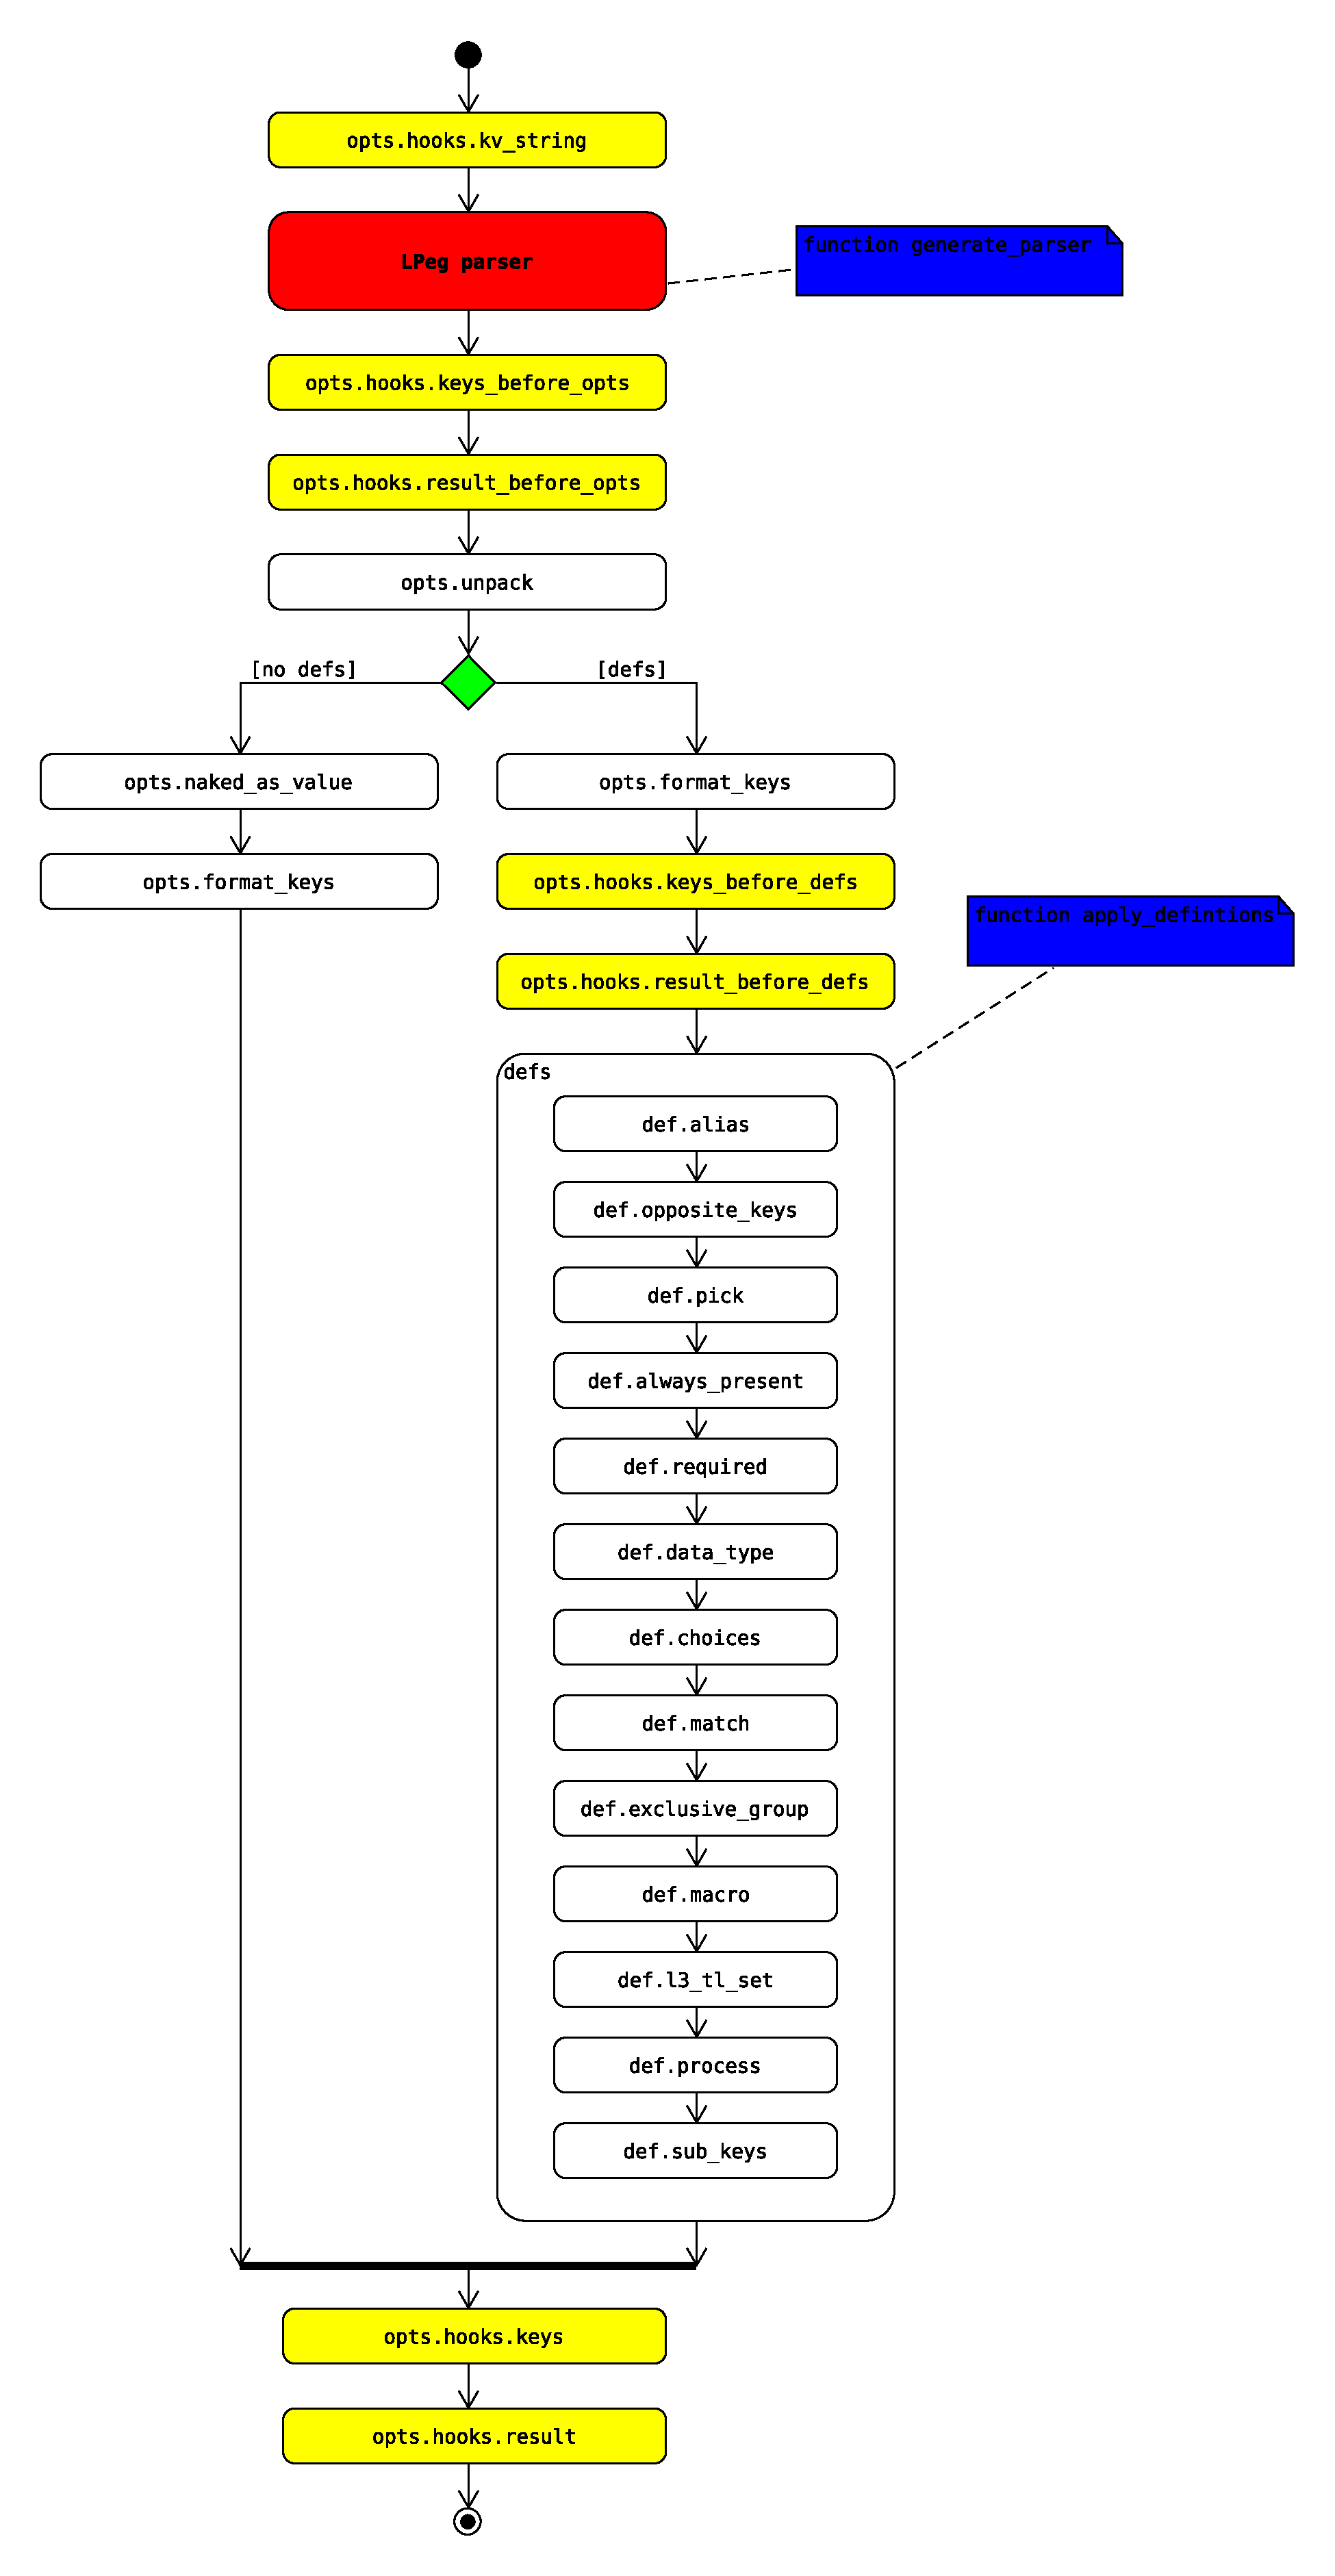
\includegraphics[width=0.8\linewidth]{Activity-Diagramm.eps}
\end{center}

%-----------------------------------------------------------------------
%
%-----------------------------------------------------------------------

\clearpage

\section{Implementation}

%%
%
%%

\subsection{luakeys.lua}

\inputminted[linenos=true]{lua}{luakeys.lua}

%%
%
%%

\clearpage

\subsection{luakeys.tex}

\inputminted[linenos=true]{latex}{luakeys.tex}

%%
%
%%

\clearpage

\subsection{luakeys.sty}

\inputminted[linenos=true]{latex}{luakeys.sty}

%%
%
%%

\clearpage

\subsection{luakeys-debug.tex}

\inputminted[linenos=true]{latex}{luakeys-debug.tex}

%%
%
%%

\clearpage

\subsection{luakeys-debug.sty}

\inputminted[linenos=true]{latex}{luakeys-debug.sty}

\changes{0.1.0}{2021/01/18}{Inital release}
\changes{0.2.0}{2021/09/19}{
* Allow all recognized data types as keys.
* Allow TeX macros in the values.
* New public Lua functions: save(identifier, result), get(identifier).
}
\changes{0.3.0}{2021/11/05}{
* Add a LuaLaTeX wrapper “luakeys.sty”.
* Add a plain LuaTeX wrapper “luakeys.tex”.
* Rename the previous documentation file “luakeys.tex” to luakeys-doc.tex”.
}
\changes{0.4.0}{2021/12/31}{
* Parser: Add support for nested tables (for example {{'a', 'b'}}).
* Parser: Allow only strings and numbers as keys.
* Parser: Remove support from Lua numbers with exponents (for example '5e+20').
* Switch the Lua testing framework to busted.
}
\changes{0.5.0}{2022/04/04}{
* Add possibility to change options globally.
* New option: standalone_as_true.
* Add a recursive converter callback / hook to process the parse tree.
* New option: case_insensitive_keys.
}
\changes{0.6.0}{2022/06/09}{
* New feature: keys now can be defined using the function
  “define(defs, opts)” or “define(kv_string, { defs = { key = { ... } } })”
* Rename the global options table from “default_options” to “opts”.
* New option “format_keys”.
* Remove option “case_insensitive_keys”. Use
  “format_keys = \{ lower \}” to achieve the same effect.
* The default value of the option “convert_dimension” is now false.
* The option “standalone_as_true” is renamed to “naked_as_value”.
  The boolean value of the option must be changed to the opposite to.
  produce the previous effect.
* The function “print()” is now called “debug()”.
}
\changes{0.7.0}{2022/07/06}{
* The project now uses semantic versioning.
* New definition attribute “pick” to pick standalone values and assign
  them to a key.
* New function “utils.scan_oarg()” to search for an optional argument,
  that means scan for tokens that are enclosed in square brackets.
* Extend and improve the documentation.
}
\changes{0.8.0}{2022/11/17}{
* Add 6 new options to change the delimiters: “assignment_operator”,
  “group_begin”, “group_end”, “list_separator”, “quotation_begin”,
  “quotation_end”.
* Extend the documentation about the option “format_keys”.
}
\changes{0.10.0}{2022/12/16}{
* The definition attibute “pick” accepts a new data type: “any”.
* The attribute value “true” for the attribute “pick” is deprecated.
* The attribute “pick” accepts now multiple data types specified in
  a table.
* Add a new function called “any(value)” in the “is” table that accepts
  any data type.
}
\changes{0.10.0}{2022/12/16}{
* Add support for an invert flat that flips the value of naked keys.
* Add new options to specify which strings are recognized as Boolean
  values.
}

\pagebreak
\PrintChanges
\pagebreak
\PrintIndex
\end{document}
